\documentclass[12pt]{article}

% MLA format
\usepackage[letterpaper]{geometry}
\usepackage{times}
\geometry{top=1.0in, bottom=1.0in, left=1.0in, right=1.0in}
\usepackage{fancyhdr}
\pagestyle{fancy}
\lhead{} 
\chead{} 
\rhead{Simmons \thepage} 
\lfoot{} 
\cfoot{} 
\rfoot{}
\renewcommand{\headrulewidth}{0pt} 
\renewcommand{\footrulewidth}{0pt} 

\usepackage{mdwlist}
\usepackage{enumitem}
\setlist{  
  listparindent=\parindent,
  parsep=0pt,
}
\title{Homework 3}
\author{Mark Simmons}
\date{February 14, 2020}

% Multi-line glosses
%\usepackage{chngcntr}
%\usepackage{gb4e,cgloss4e}

%\newcounter{glossnum}

%\newcommand{\numgloss}{\refstepcounter{glossnum}\alph{glossnum}.\space}
%\counterwithin{glossnum}{xnumi}
%\renewcommand{\theglossnum}{\thexnumi\alph{glossnum}}

% Typing in IPA
\usepackage{tipa}

% Sentence trees
\usepackage{tikz-qtree}
\usepackage{lscape}
\usepackage{graphicx}
\tikzset{level distance=30pt,
    sibling distance=6pt,
    every tree node/.style={align=center},
    }

\begin{document}

\maketitle

\begin{enumerate}

% question 1
\item Argumentation


The following two sentences each have what appear to be verb phrases with prepositional phrase arguments following the verb.

\begin{enumerate}
\item She looked down the canyon.
\item She blew off her homework.
\suspend{enumerate}

I argue that sentence (b), though at a phonological level appears to have the same structure as (a), is better analyzed syntactically as a single verb constituent consisting of two orthographically distinct morphemes, i.e. a ``phrasal verb.'' This hypothesis predicts that ``homework'' is the daughter of the verb phrase headed by ``blow off'' while ``the canyon'' is the daughter of the prepositional phrase headed by ``down.'' To prove this point, I will demonstrate that ``blow off'' performs better in various constituent tests than ``look down.'' I will also argue that the semantics of sentence (a) make the analysis of ``blow off'' as a phrasal verb preferable to the a mere union of the semantics of ``blow'' and ``off,'' and that such is not the case for ``look down.''

In an argument alternation constituency test, sentence (b) performs better than (a) (note that I changed the determiner ``her'' to ``the'' for sentence (b) to make the semantics more natural, but this should have no bearing on the syntax of the VP or the sentence in general).

\resume{enumerate}
\item ??The canyon was looked down by her.
\item ?The homework was blown off by her.
\suspend{enumerate}

Since, semantically, all passive sentences with an inanimate subject and animate agent are problematic for English speakers, removing the agent from the sentences makes the distinction clear.

\resume{enumerate}
\item *The canyon was looked down.
\item The homework was blown off.
\suspend{enumerate}

The ungrammaticality of ``look down'' without a noun phrase that could function as the sister of the preposition ``down'' suggests that the two words do not form a single constituent. ``blow off,'' on the other hand, is acceptable without any NP dominated by the VP.

``Blow off'' can also be replaced easily by a single verb of similar semantics, whereas the same cannot be done for ``look down.''
\resume{enumerate}
\item *She gazed the canyon.
\item She disregarded her homework.
\suspend{enumerate}

The best grammatical single-replacement for ``look down'' in sentence (a) could be ``She saw the canyon,'' but this does not have the same semantics of ``look down'' (namely, the direction of her looking/seeing), whereas ``blow off'' can easily be replaced by ``disregard'' without any loss of semantics clearly resulting from losing the preposition ``off.''

The standalone test demonstrates that ``look'' can be disassociated from the preposition ``down'' while doing so is unacceptable for ``blow off.''
\resume{enumerate}
\item What did she do down the canyon?\\
-She looked.
\item *What did she do off her homework?\\
-She blew.
\suspend{enumerate}

It bears note that, semantically, ``look down'' is a perfect composite of the semantics of ``look'' (intentionally perceive with the eyes) and ``down'' (with downward or descending direction.) ``Blow off'', however, is unrelated to the literal semantics of either component. It's meaning of ``shirk or disregard'' does not comprise any forceful expulsion of air (blow), nor does it have any directional or spacial component to it. In other words, any semantic relation ``blow off'' has to its components is figurative and idiomatic, which suggests it is a fixed expression.

Other verb-preposition pairs canonically considered ``phrasal verbs'' have similar semantics.
\resume{enumerate}
\item She ran out of ideas.
\item She gets along with her roommate.
\suspend{enumerate}

``Run out,'' for example, involves nether locomotion (run) or direction away from a location of reference (out). Neither does ``get along'' involve any literal reception or obtaining on behalf of the agent (get), or progressive motion following or accompanying another entity (along).

Sentence (b) can be paraphrased as ``she shirked her responsibility to complete her homework.'' No preposition is needed as sister of ``her homework.'' The other phrasal verbs can likewise be paraphrased without any preposition adjacent to the object (sentence (n) still needs the preposition ``with'', present in the original, but note that ``along'' has disappeared with no equivalent preposition to take its place.)
\resume{enumerate}
\item She exhausted all her ideas.
\item She has a good relationship with her roommate.
\suspend{enumerate}

Any paraphrase of sentence (a) still requires an equivalent preposition (or relational noun, in sentence (p) to convey similar semantics.

\resume{enumerate}
\item She gazed along the canyon.
\item  She visually inspected the length of the canyon.
\suspend{enumerate}

Together, these arguments show that the semantic strucure and syntactic patterning of ``blow off'' in sentence (b) favors analysis as a single constituent phrasal verb, whereas ``look down'' is best analyzed as two independent morphemes.

% question 2
\item Sentence Trees


\begin{enumerate}
\item \leavevmode\vadjust{\vspace{-\baselineskip}}\newline
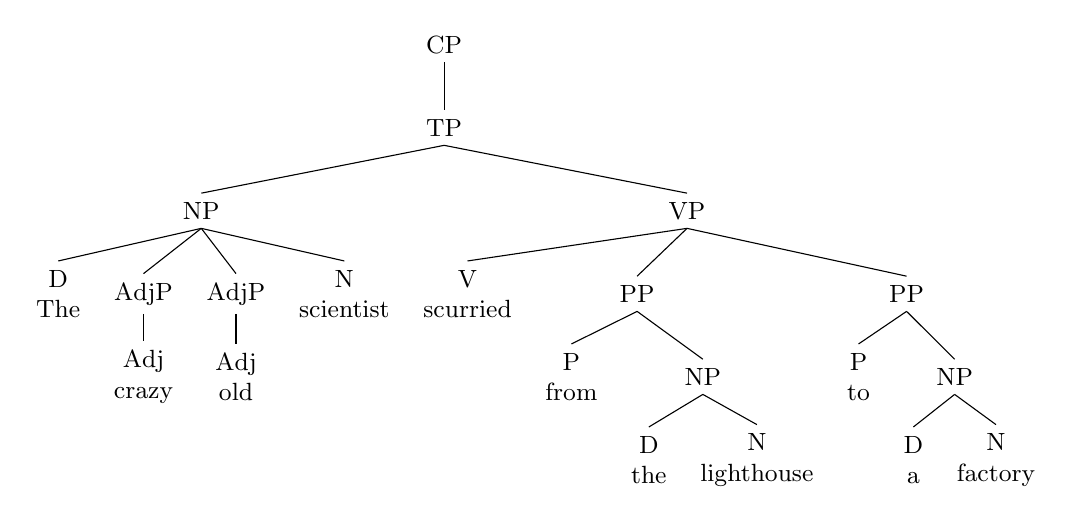
\begin{tikzpicture}
{\small \Tree 
[.CP 
[.TP 
	[.NP D\\The [.AdjP Adj\\crazy ] [.AdjP Adj\\old ]  N\\scientist ]
	[.VP V\\scurried
		[.PP P\\from [.NP D\\the N\\lighthouse ] ]
		[.PP P\\to [.NP D\\a N\\factory ] ]
	]
]
]
}\\
\end{tikzpicture}

\item \leavevmode\vadjust{\vspace{-\baselineskip}}\newline
%\begin{landscape}
\noindent\resizebox{\textwidth}{!}{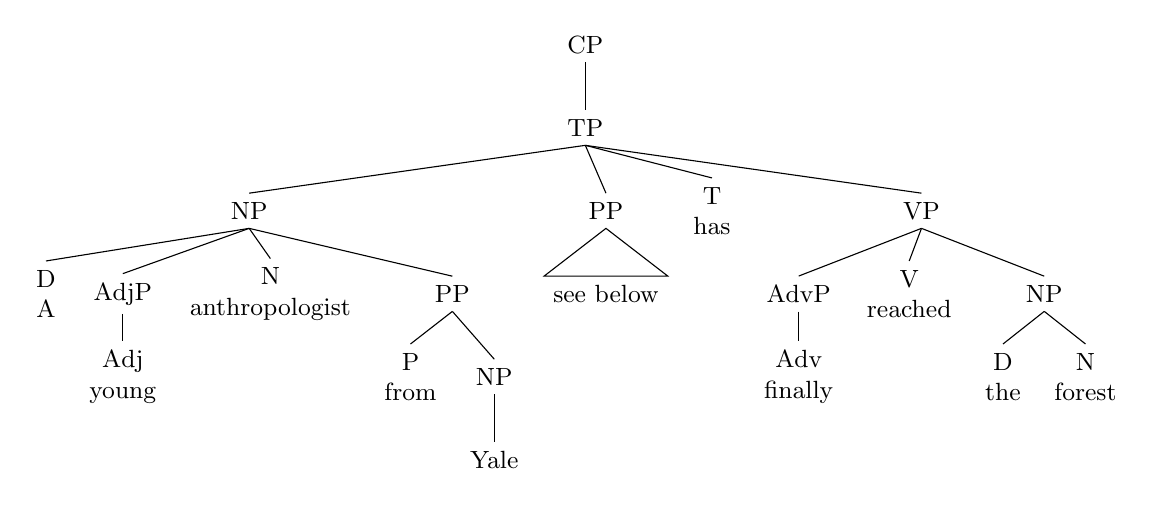
\begin{tikzpicture}
{\small \Tree
[.CP
[.TP
	[.NP D\\A
		[.AdjP Adj\\young ]
		N\\anthropologist
		[.PP P\\from
			[.NP Yale ]
		]
	]
	[.\node(PP){PP}; \edge[roof]; {see below} ]
	T\\has
	[.VP
		[.AdvP Adv\\finally ]
		V\\reached
		[.NP D\\the N\\forest ]
	]
]
]
}
\end{tikzpicture}}
%\end{landscape}
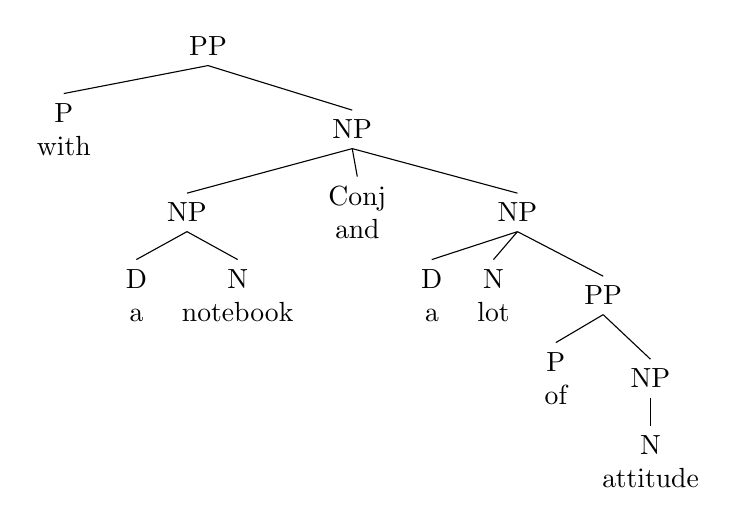
\begin{tikzpicture}
\Tree
[.PP P\\with
	[.NP [.NP D\\a N\\notebook ]
	Conj\\and
	[.NP D\\a N\\lot
		[.PP P\\of [.NP N\\attitude ] ]
	] ]
]
\end{tikzpicture}

\item \leavevmode\vadjust{\vspace{-\baselineskip}}\newline
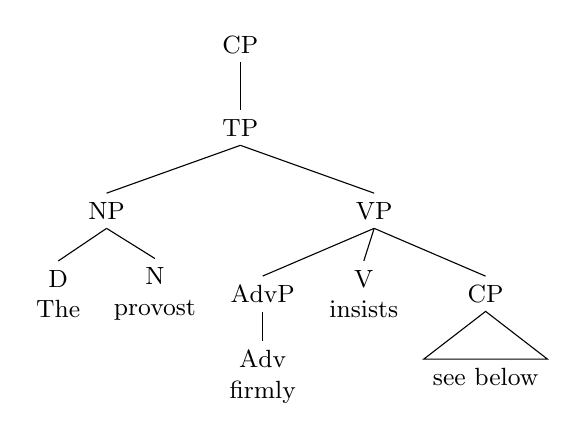
\begin{tikzpicture}
{\small \Tree
[.CP
[.TP
	[.NP D\\The N\\provost ]
	[.VP
		[.AdvP Adv\\firmly ]
		V\\insists
		[.\node(CP){CP}; \edge[roof]; {see below} ]
	]
]
]
}
\end{tikzpicture}

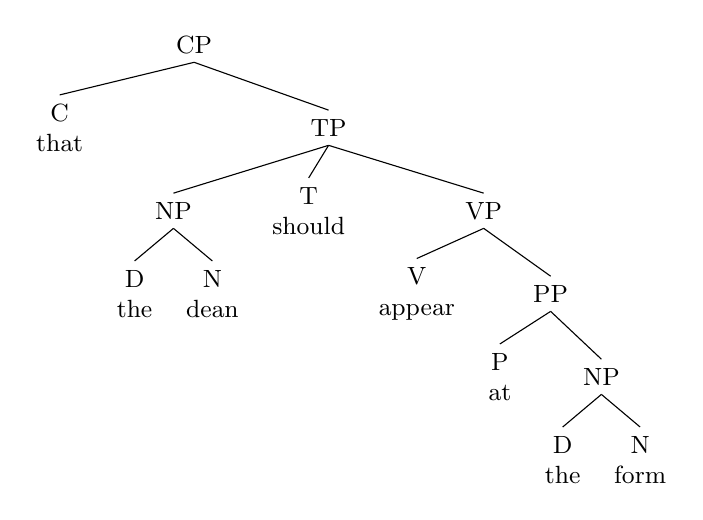
\begin{tikzpicture}
{\small \Tree
[.CP
C\\that
[.TP
	[.NP D\\the N\\dean ]
	T\\should
	[.VP V\\appear
		[.PP P\\at
			[.NP D\\the N\\form ]
		]
	]
]
]
}
\end{tikzpicture}

\item This sentence can have one of two meanings. It can be interpreted as ``James very silently read an English poem that was old.''\\
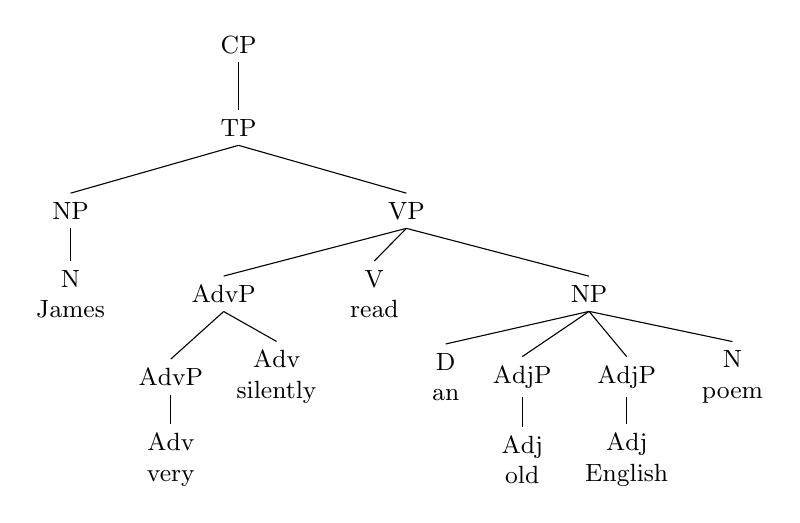
\begin{tikzpicture}
{\small \Tree
[.CP
[.TP
	[.NP N\\James ]
	[.VP
		[.AdvP
			[.AdvP Adv\\very ]
			Adv\\silently
		]
		V\\read
		[.NP D\\an
			[.AdjP Adj\\old ]
			[.AdjP Adj\\English ]
			N\\poem
		]
	]
]
]
}
\end{tikzpicture}


It can also be read as ''James very silently read a poem written in Old English.''

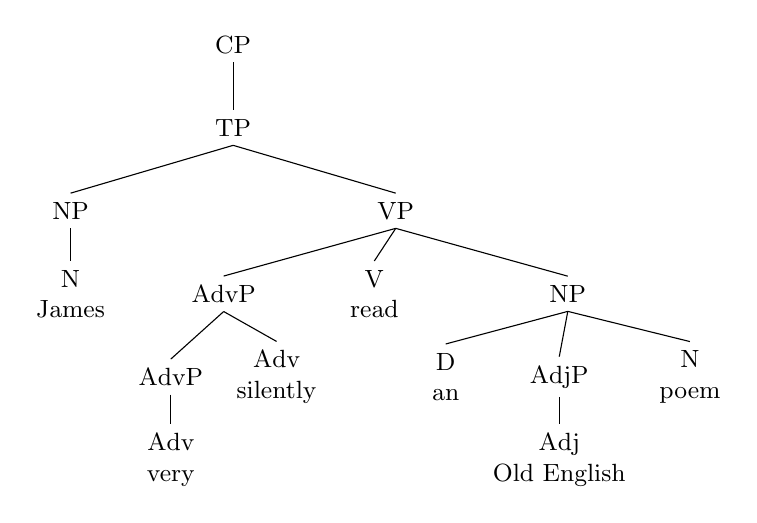
\begin{tikzpicture}
{\small \Tree
[.CP
[.TP
	[.NP N\\James ]
	[.VP
		[.AdvP
			[.AdvP Adv\\very ]
			Adv\\silently
		]
		V\\read
		[.NP D\\an
			[.AdjP Adj\\{Old English} ]
			N\\poem
		]
	]
]
]
}
\end{tikzpicture}

\end{enumerate}

% question 3
\item Indonesian Syntax
\begin{enumerate}

\item Affirmative imperatives are formed from the uninflected verb root at the onset of the sentence with any direct objects following. Negative imperatives seem to be formed with negative particle {\it jangan} preceding the verb, but are otherwise identical to affirmative imperatives.

\item Negative declaratives are formed with the negative particle {\it tidak} before the verb, but are otherwise identical to affirmative declaratives.

\item Affirmative polar questions are formed with the interrogative particle {\it apa} at the beginning of the sentence, but are otherwise identical in structure to affirmative declarative sentences. Negative polar questions could possible be formed with {\it apa} at sentence onset, and the negative particle {\it tidak} preceding the verb. Under this hypothesis "Does Ms. Epps not listen to music?" would be {\it Apa Mas Epps tidak mendengar musik?}

\item The verbs in (3) all share a prefix {\it meng-}, with allomorphs {\it men-} and {\it mem-}, assimilating to the place of articulation of the onset consonant of the verb root. The verbs in (4) all lack this prefix.

\item Judging by this corpus, {\it meng-} appears to be a prefix marking transitive declarative verbs. Thus, I would hypothesize that any verb found bearing this prefix likely has a transitive sense.

\item Past tense of verbs appears to be unmarked in Indonesian. All declarative sentences given in this corpus have both past and present readings in English, suggesting that Indonesian does not distinguish between those tense features through any overt marking. Plurality is less certain. The only noun seen thus far which is semantically plural is {\it kercis} "tickets." Since the same word is not seen in a singular sense, we can make no assumptions about how nominal plurals are formed in Indonesian, except that there does not appear to be a lexically independent morpheme to mark plural (cf., for example, Kaqchikel "taq chay" (PL house) ).

\item Assignment 1 demonstrated the determiners indicating possession (e.g. {\it saya} 1s) and demonstrative deixis (e.g. {\it ini} proximal demonstrative) occur after the noun. This assignment demonstrates that, in pragmatic contexts that condition definite articles in English (I bought/buy {\bf the} tickets), no determiner occurs in Indonesian (Saya membeli kercis). It thus appears from these data that determiners do not perform the role of marking definiteness of noun phrases.

\end{enumerate}

\end{enumerate}



\end{document}
